\section{Design the EKF time update step}

\subsection{Task 3}

To derive a discretized model from the continuous time model in equation (5), we can solve the differential equation and use the relation $exp(A) \approx I + A$ to obtain the discretized form. Here's the derivation:

The continuous time model is :
\begin{equation}
    \begin{aligned}
        \dot q(t)=\frac12S\left(w_{k-1}+v_{k-1}\right)q(t)
    \end{aligned}
\end{equation}

Use the relation $exp(AΔt) \approx I + AΔt$ to solve ODE:

\begin{equation}
    \begin{aligned}
        q(t+T)=\exp\left(\frac{1}{2}S\left(w_{k-1}+v_{k-1}\right)T\right)\cdot q(t) = \left[\mathbf{I}+{\frac{T}{2}}S\left(w_{k-1}+v_{k-1}\right)\right]\cdot q(t)\\
    \end{aligned}
\end{equation}

$T $ is the sample time interval. And the form can be translated into a discretized style:

\begin{equation}
    \begin{aligned}
        q_k&=\mathbf{I}\cdot q_{k-1}+\frac{T}{2}S\left(w_{k-1}+v_{k-1}\right)\cdot q_{k-1}\\
        &=\left(\mathbf{I}+{\frac{T}{2}}S\left(w_{k-1}\right)\right)\cdot q_{k-1}+{\frac{T}{2}}S\left(v_{k-1}\right)\cdot q_{k-1}
    \end{aligned}
\end{equation}

So we get:
\begin{equation}
    \begin{aligned}
        F(\omega_{k-1}) = \mathbf{I}  + \frac{T}{2}\cdot S(\omega_{k-1})\\
G(\hat{q}_{k-1}) = \frac{T}{2} \cdot S(\hat{q}_{k-1})\\
    \end{aligned}
\end{equation}




\subsubsection{Reason for Discretize}

In the EKF, the prediction step involves propagating the state estimate and covariance from the previous time step to the current time step. This propagation is typically done using the continuous-time dynamic model, which can be linearized around the current state estimate. However, linearizing the model can introduce errors, especially for highly nonlinear systems.

To address this issue, the discretized model derived using the approximation techniques provides an alternative approach for the prediction step in the EKF. By discretizing the continuous-time dynamic model, we can directly apply it in the discrete-time domain without the need for linearization.

\subsection{Task 4}

If there are angular velocities, update the estimate and covariance as motion model, in function \texttt{tu\_qw}.

Once $ v_k $ is missing, use the same consideration as in homework 2, skip the update for the current time, and keep the state and covariance value as the latest update value.

\subsection{Task 5}

In the function \texttt{Task5\_filterTemple}, I utilized the \texttt{tu\_qw } and \texttt{mu\_normalizeQ} functions for the gyroscope sensor.

As observed and analyzed previously, the gyroscope provides accurate angular velocities but cannot obtain the absolute orientation.

To address this, I established the initial flat state by starting with the phone facing left and standing on its left edge. However, during the process, it consistently exhibits an offset compared to the orientation measurement, which is displayed as 'Google'.

Additionally, the gyroscope is prone to drifting due to this bias. To demonstrate this behavior, I conducted a procedure where I placed the phone on a table, shook it for a period of time, and then returned it to its original position. I repeated this procedure twice, and the resulting drift process is clearly depicted in Figure \ref{fig:drift-process}.

\begin{figure}[H]
    \centering
    \begin{subfigure}[H]{0.3\textwidth}
        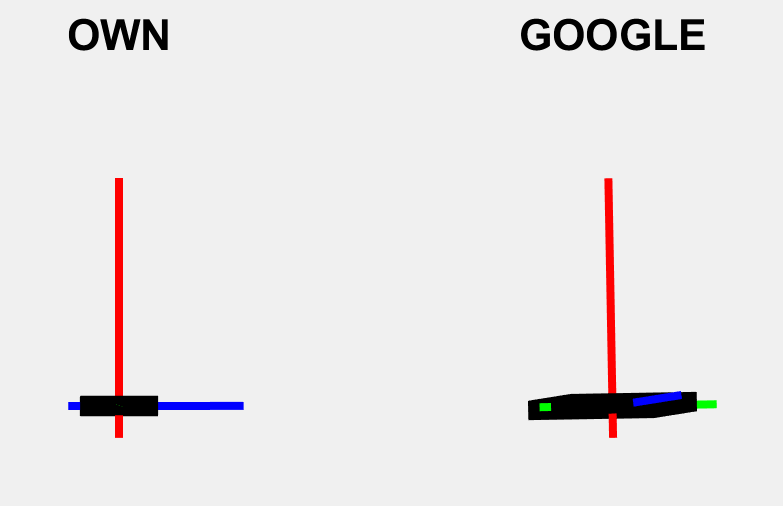
\includegraphics[width=\textwidth]{images/beginning.png}
        \caption{Begin}
        \label{fig:begin}
    \end{subfigure}
    \hfill
    \begin{subfigure}[H]{0.3\textwidth}
        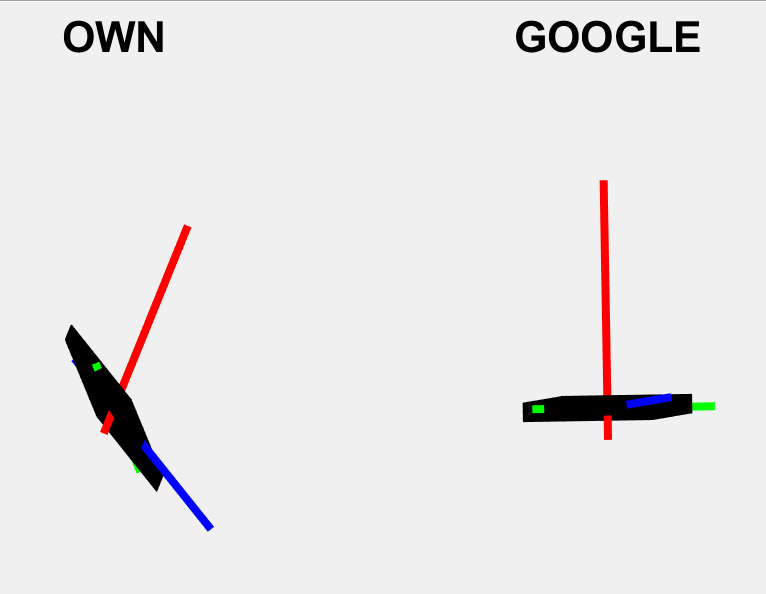
\includegraphics[width=\textwidth]{images/drift1.png}
        \caption{Firstshake}
        \label{fig:drift1}
    \end{subfigure}
    \hfill
    \begin{subfigure}[H]{0.3\textwidth}
        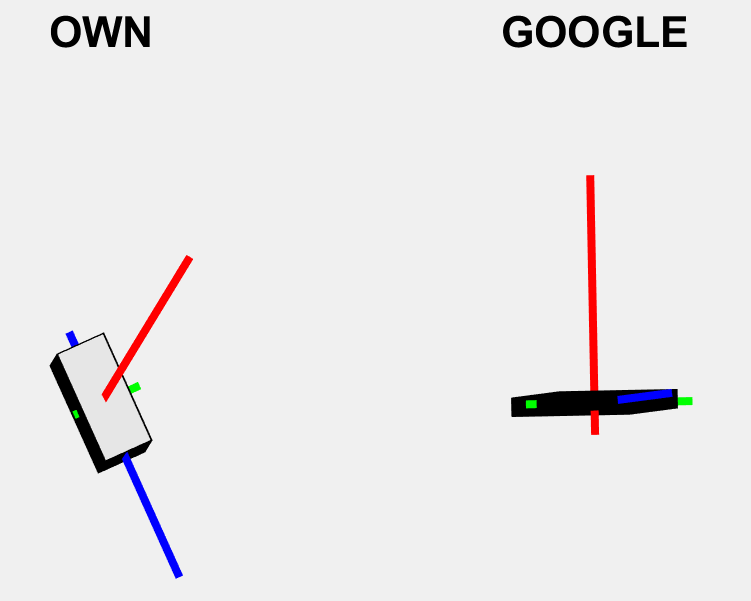
\includegraphics[width=\textwidth]{images/drift2.png}
        \caption{Secondshake}
        \label{fig:drift2}
    \end{subfigure}
    \caption{Drift Process}
    \label{fig:drift-process}
\end{figure}



